%%%%%%%%%%%%%%%%%%%%%%%%%%%%%%%%%%%%%%%%%%%%%%%%%%%%%%%%%%%%%%%%%%%%%%%%%%%%%%%%%%%%%%%%%%%%%%%%%%%%%%%%%%%%%%%%%%
%%  DRAFT: affiliations, keywords and the declaration of interests are still to be filled in before submission.
%%
%%  AUTHORSHIP: Johan Bjoerk, the original author of the Nervus software, agreed to be an author on 2026-11-25.
%%
%%  Class file: jfm.cls from the Cambridge University Press JFM author template. Its licence allows its use only
%%  for articles to be published by Cambridge University Press, so it is not in the repository: see README.md.
%%
%%  Every number in the text comes from numbers.tex, which make_numbers.py writes from results.json, which
%%  analysis.py writes. Rebuild: uv run python paper/analysis.py && uv run python paper/make_numbers.py
%%%%%%%%%%%%%%%%%%%%%%%%%%%%%%%%%%%%%%%%%%%%%%%%%%%%%%%%%%%%%%%%%%%%%%%%%%%%%%%%%%%%%%%%%%%%%%%%%%%%%%%%%%%%%%%%%%
\RequirePackage{fix-cm}  % scalable Computer Modern at the class's 10.5 pt
\documentclass{jfm}
\setlength{\paperwidth}{210mm}  % jfm.cls sets no paper size; A4 for the PDF only
\setlength{\paperheight}{297mm}
\usepackage{graphicx}
\usepackage{natbib}
\usepackage{booktabs}
\usepackage{array}
\usepackage{amsmath}
\usepackage[colorlinks=true,urlcolor=blue,citecolor=black,linkcolor=black]{hyperref}
% Generated by make_numbers.py from results.json. Do not edit.
\newcommand{\NervusVersion}{0.1.0}
\newcommand{\Cfit}{0.680}
\newcommand{\CfitNinety}{0.680}
\newcommand{\CfitSeventyFive}{0.686}
\newcommand{\AreaTop}{129.0}
\newcommand{\AreaBottom}{103.0}
\newcommand{\RTop}{1.69}
\newcommand{\RBottom}{1.34}
\newcommand{\Ro}{0.0992}
\newcommand{\HCountsMin}{1.89}
\newcommand{\TrainN}{6\,717}
\newcommand{\TestN}{6\,771}
\newcommand{\TrainNfit}{5\,656}
\newcommand{\TestNwin}{5\,702}
\newcommand{\TrainTend}{1091}
\newcommand{\TestTend}{1092}
\newcommand{\TrainTcut}{901}
\newcommand{\TestTcut}{909}
\newcommand{\TrainHcut}{3.07}
\newcommand{\TestHcut}{3.19}
\newcommand{\TrainHzero}{26.55}
\newcommand{\TestHzero}{26.49}
\newcommand{\TrainRMSE}{0.33}
\newcommand{\TrainMAE}{0.26}
\newcommand{\TrainMax}{1.14}
\newcommand{\TrainAllRMSE}{0.33}
\newcommand{\TrainAllMax}{1.14}
\newcommand{\TestRMSE}{0.43}
\newcommand{\TestMAE}{0.36}
\newcommand{\TestMax}{1.08}
\newcommand{\TestBias}{$-0.30$}
\newcommand{\TestAllRMSE}{0.43}
\newcommand{\TestAllMAE}{0.37}
\newcommand{\TestAllMax}{1.08}
\newcommand{\TrainDSMAE}{0.25}
\newcommand{\TestDSMAE}{0.34}
\newcommand{\TrainTthreeModel}{887}
\newcommand{\TrainTthreeData}{903}
\newcommand{\TestTthreeModel}{885}
\newcommand{\TestTthreeData}{919}
\newcommand{\VerAuto}{3.8e-06}
\newcommand{\VerRKfour}{9.4e-07}
\newcommand{\VerScipy}{5.0e-06}
\newcommand{\VerTempty}{1266}
\newcommand{\RhoAir}{1.163}
\newcommand{\ResidCorr}{0.94}
\newcommand{\ResidBins}{44}
\newcommand{\CdEighth}{0.27}
\newcommand{\SlantFactor}{0.9998}
\newcommand{\LevelDrop}{23}
\newcommand{\CalibSplineMax}{9.2}
\newcommand{\CalibSplineRMS}{3.8}
\newcommand{\CalibStepMedian}{9.0}
\newcommand{\CalibStepMax}{37}
\newcommand{\RhoTempLow}{14}
\newcommand{\RhoTempHigh}{34}
\newcommand{\CdHandoutFiftyK}{0.41}
\newcommand{\CdMisprintFiftyK}{0.92}
\newcommand{\GlobeMeanErr}{$-0.75$}
\newcommand{\GlobeMAE}{0.75}
\newcommand{\GlobeMax}{0.80}
\newcommand{\GlobeRel}{$-9.5$}
\newcommand{\GlobeReMin}{8.1}
\newcommand{\GlobeReMax}{9.3}
\newcommand{\GlobeCdEff}{0.54}
\newcommand{\GlobeCdEffMin}{0.52}
\newcommand{\GlobeCdEffMax}{0.56}
\newcommand{\GlobeCdModel}{0.42}
\newcommand{\GlobeCdRatio}{28}
\newcommand{\GlobeVRatioMin}{100.0}
\newcommand{\GlobeTninetyFive}{31}
\newcommand{\BladderMeanErr}{$-2.01$}
\newcommand{\BladderMAE}{2.01}
\newcommand{\BladderMax}{2.75}
\newcommand{\BladderRel}{$-10.2$}
\newcommand{\BladderReMin}{3.7}
\newcommand{\BladderReMax}{4.7}
\newcommand{\BladderCdEff}{0.51}
\newcommand{\BladderCdEffMin}{0.47}
\newcommand{\BladderCdEffMax}{0.54}
\newcommand{\BladderCdModel}{0.40}
\newcommand{\BladderCdRatio}{25}
\newcommand{\BladderVRatioMin}{100.0}
\newcommand{\BladderTninetyFive}{8}
\newcommand{\MercTmin}{3.75}
\newcommand{\MercTmax}{3.75}
\newcommand{\MercReMin}{4.2}
\newcommand{\MercReMax}{4.6}
\newcommand{\TvacThirteen}{3.70}
\newcommand{\TvacFourteen}{4.11}
\newcommand{\SensSpreadMax}{1.10}
\newcommand{\GlobeSensUp}{0.20}
\newcommand{\GlobeMinDeficit}{0.68}
\newcommand{\BladderSensUp}{0.99}
\newcommand{\BladderMinDeficit}{1.33}
\newcommand{\SensReached}{0}
\newcommand{\SensReachedText}{none of them brings any of the eleven light objects up to its measured time}
\newcommand{\MercT}{3.75}
\newcommand{\EulerOrder}{1.02}
\newcommand{\RKOrder}{4.00}
\newcommand{\RKFFSlope}{1.01}
\newcommand{\StabExact}{57.830}
\newcommand{\StabSim}{57.826}
\newcommand{\SatErrOn}{$3.6\times10^{-9}$}
\newcommand{\SatErrOff}{$1.9\times10^{-6}$}
\newcommand{\SilDiff}{$2.2\times10^{-16}$}
\newcommand{\SilSteps}{2\,000}
\newcommand{\FixLSB}{0.4997}
\newcommand{\HydTHalf}{0.197}
\newcommand{\StPaulsRows}{%
13 & Hg globe 1 & 58.8 & 20 & 4 & 3.75 & -- & 4.5 & -- \\
13 & Hg globe 2 & 63.7 & 20 & 4$^-$ & 3.75 & -- & 4.6 & -- \\
13 & Hg globe 3 & 56.1 & 20 & 4 & 3.75 & -- & 4.5 & -- \\
13 & Hg globe 4 & 48.4 & 19 & 4$^+$ & 3.75 & -- & 4.2 & -- \\
13 & Hg globe 5 & 52.4 & 19 & 4 & 3.75 & -- & 4.3 & -- \\
13 & Hg globe 6 & 50.8 & 19 & 4$^+$ & 3.75 & -- & 4.3 & -- \\
13 & glass globe 1 & 33.0 & 130 & 8.50 (8.20) & 7.42 & $-0.78$ & 8.4 & 0.53 \\
13 & glass globe 2 & 41.6 & 132 & 8.00 (7.70) & 6.90 & $-0.80$ & 9.3 & 0.56 \\
13 & glass globe 3 & 38.8 & 130 & 8.00 (7.70) & 6.97 & $-0.73$ & 9.0 & 0.54 \\
13 & glass globe 4 & 33.4 & 127 & 8.25 (7.95) & 7.27 & $-0.68$ & 8.4 & 0.52 \\
13 & glass globe 5 & 31.3 & 127 & 8.50 (8.20) & 7.46 & $-0.74$ & 8.1 & 0.53 \\
13 & glass globe 6 & 41.5 & 132 & 8.00 (7.70) & 6.90 & $-0.80$ & 9.3 & 0.56 \\
14 & bladder 1 & 8.3 & 134 & 19.00 & 17.18 & $-1.82$ & 4.3 & 0.50 \\
14 & bladder 2 & 10.1 & 132 & 17.00 & 15.40 & $-1.60$ & 4.7 & 0.50 \\
14 & bladder 3 & 8.9 & 135 & 18.00 & 16.67 & $-1.33$ & 4.4 & 0.47 \\
14 & bladder 4 & 6.3 & 134 & 22.00 & 19.46 & $-2.54$ & 3.7 & 0.52 \\
14 & bladder 5 & 6.4 & 127 & 21.12 & 18.38 & $-2.75$ & 3.8 & 0.54 \\}
\newcommand{\VerRows}{%
Solvers & first-order lag, unit step & $1-\mathrm{e}^{-t/\tau}$ & $2.0\times10^{-11}$ \\
 & second-order system, $\zeta = 0.2$ & closed form & $5.2\times10^{-11}$ \\
 & Euler, $h = 0.1/2^k$ & observed order & 1.02 \\
 & Runge--Kutta 4, $h = 0.1/2^k$ & observed order & 4.00 \\
Events & thrown body on an integrator limit & impact time & $0$ s \\
 & integral of a saturated sine & closed form & $3.6\times10^{-9}$ \\
Discrete & PI loop, $T = 10$ ms and 25 ms & exact $z$-domain recursion & $7.4\times10^{-13}$ rad/s \\
 & stability limit (pole at $z=-1$) & 57.830 ms & 0.005 ms \\
Physical & RC circuit & exponential & $9.8\times10^{-9}$ V \\
 & series RLC circuit & damped sine & $1.4\times10^{-11}$ A \\
 & thermal capacity cooling & exponential & $8.1\times10^{-10}$ K \\
 & inertia, damper, torque & exponential & $5.9\times10^{-10}$ rad/s \\
 & volume filled through an orifice & implicit closed form & $1.1\times10^{-10}$ bar \\
Fluid & Torricelli draining, constant area & closed form & $3.8\times10^{-6}$ cm \\
 & sphere, constant $C_D$: speed & $v_t \tanh(t/T)$ & $4.4\times10^{-13}$ m/s \\
 & sphere, constant $C_D$: height & $v_t T \ln\cosh(t/T)$ & $2.0\times10^{-13}$ m \\
Linear & Bode, $1/(0.5s+1)$ & magnitude, phase & $3.6\times10^{-15}$ dB, $1.4\times10^{-14}$$^\circ$ \\
 & margins, $1/(s(s+1))$ & PM 51.827$^\circ$, GM $\infty$ & $2.9\times10^{-7}$$^\circ$, -- \\
 & margins, $10/(s(s+1)(0.1s+1))$ & PM 1.576$^\circ$, GM $0.828$ dB & $7.1\times10^{-7}$$^\circ$, $3.9\times10^{-7}$ dB \\
 & margins, $(s+1)^2/s^3$ & PM 21.386$^\circ$, GM $-6.021$ dB & $1.0\times10^{-6}$$^\circ$, $1.2\times10^{-6}$ dB \\
Code & generated C vs.\ simulation & identical & $2.2\times10^{-16}$ \\
 & fixed point, fixdt(1,16,8) & $\le$ 1/2 LSB & 0.4997 LSB \\}


\shorttitle{Lumped fluid models in a block-diagram simulator}
\shortauthor{N. Nordin and J. Bjoerk}

\title{Lumped-parameter fluid dynamics in a block-diagram simulator: validation against orifice draining of a
tank and Newton's falling spheres}

\author{Niklas Nordin\aff{1}\corresp{\email{niklas.nordin@nequam.se}}
 \and Johan Bjoerk\aff{2}}

\affiliation{\aff{1}[Affiliation to be confirmed]
\aff{2}[Affiliation to be confirmed]}

\begin{document}

\maketitle

\begin{abstract}
Block-diagram simulators are widely used for zero-dimensional models of fluid systems, but their comparison with
measurements is rarely documented in a repeatable form. We verify Nervus, an open-source block-diagram simulator
written in Python, against exact solutions module by module, and then validate it against two published data sets.
The first is the gravity draining of a tank through a small side orifice, with a calibration run and a replicate
run \citep{Fabusola2025}. A discharge coefficient fitted to the calibration run, $C_d = \Cfit$, predicts the
replicate run with a root-mean-square error of \TestRMSE~cm over a \LevelDrop~cm fall in level. The residuals of
the two runs are strongly correlated as functions of the level (correlation coefficient \ResidCorr), pointing to the
level-sensor calibration rather than the flow model. The second is the drop experiments made from the dome of
St~Paul's Cathedral in 1710 and 1719 and tabulated by \citet{Newton1726}. With a steady-sphere drag correlation and
no fitted parameter, the simulated falls of six glass globes and five inflated bladders are systematically short,
by \GlobeMeanErr~s (\GlobeRel\%) and \BladderMeanErr~s (\BladderRel\%) on average; matching the measured times
requires effective drag coefficients \GlobeCdRatio\% and \BladderCdRatio\% above the correlation, more than
plausible changes to the model inputs explain. In the verification cases (convergence orders of the solvers, event
location, a discrete stability limit, physical networks, stability margins and generated C code) the errors are
orders of magnitude below these discrepancies.
\end{abstract}

\begin{keywords}
% JFM keywords are chosen from the journal's list during online submission. These are placeholders to be
% replaced with terms from that list.
low-dimensional models, wakes
\end{keywords}

%%%%%%%%%%%%%%%%%%%%%%%%%%%%%%%%%%%%%%%%%%%%%%%%%%%%%%%%%%%%%%%%%%%%%%%%%%%%%%%%%%%%%%%%%%%%%%%%%%%%%%%%%%%%%%%%%%
\section{Introduction}\label{sec:intro}

Much of the fluid mechanics in engineering practice is done with lumped, zero-dimensional models: a tank is a
level, an orifice is a discharge coefficient, a falling body is a velocity and a drag law. In the automotive,
process and aerospace industries such models are usually assembled as block diagrams in graphical simulators, in
which integrators, gains and nonlinear functions are wired into a system of ordinary differential equations that
a library solver integrates. The physics in these models is classical; what is less often examined is whether the
simulator, the modelling conventions it encourages and the published data agree quantitatively, and how much of
any disagreement belongs to the model, to the numerics and to the measurements.

This paper reports such a comparison for Nervus \citep{Nervus}, an open-source block-diagram simulator written in
Python. We chose two cases that test different things. The first, the draining of a tank through a small side
orifice \citep{Fabusola2025}, is a modern laboratory data set with thousands of samples, a calibration run and a
replicate run. It allows the textbook separation of calibration from validation: one parameter is fitted to one
run and the other run is predicted. The second, the drop experiments made from the dome of St~Paul's Cathedral in
London in 1710 and 1719 and tabulated by Newton in the third edition of the \emph{Principia}
\citep{Newton1726,Newton1846}, is historical. Only total fall times were measured, but every parameter of a
modern drag model is fixed by the tabulated weights and diameters, so the comparison involves no fitting at all.
We are not aware of a published re-analysis of Newton's table with a modern sphere-drag correlation, but we make
no claim that none exists.

Section~\ref{sec:nervus} describes the simulator as far as it matters here. Following the usual hierarchy,
\S\,\ref{sec:verification} first verifies the software against exact solutions, module by module; then
sections~\ref{sec:tank} and~\ref{sec:drops} present the two validation cases, \S\,\ref{sec:discussion} discusses the sources of error, and
\S\,\ref{sec:conclusions} concludes.

%%%%%%%%%%%%%%%%%%%%%%%%%%%%%%%%%%%%%%%%%%%%%%%%%%%%%%%%%%%%%%%%%%%%%%%%%%%%%%%%%%%%%%%%%%%%%%%%%%%%%%%%%%%%%%%%%%
\section{The simulator}\label{sec:nervus}

A Nervus model is a directed graph of blocks. Each block is a small dynamical system with inputs, outputs,
parameters and, possibly, continuous or discrete states; the wires carry signals between output and input ports.
A continuous state is introduced by an integrator block, whose output is the state and whose input its time
derivative. Parameters may be numbers or expressions of named variables held in a model workspace, so that one
model can be run with different parameter values without being edited. Nonlinear functions that are not
available as library blocks can be written as stateless Python functions in a \emph{Python Function} block. The
models used here consist of integrators, sums, gains, a saturation, a square root, a product and one Python
Function block each; they are stored as plain JSON files and can be built either in the graphical editor or from a
Python script, as here.

Before a run, the diagram is compiled: blocks are sorted into an execution order that respects direct
feedthrough, and the continuous states of all integrators are gathered into one state vector. Continuous states
are integrated by the variable-step solvers of SciPy \citep{Virtanen2020}, by default the fifth-order
Dormand--Prince pair \citep{Dormand1980}, or by fixed-step explicit Euler and classical fourth-order Runge--Kutta
methods implemented in Nervus. With variable-step solvers, blocks with discontinuities (such as the saturation in
the tank model) declare zero-crossing functions, and the solver locates their roots so that steps do not straddle a
change of mode. All results below were computed with the development version of Nervus that follows release
\NervusVersion; unless stated otherwise, the relative and absolute tolerances were $10^{-9}$ and $10^{-11}$.

%%%%%%%%%%%%%%%%%%%%%%%%%%%%%%%%%%%%%%%%%%%%%%%%%%%%%%%%%%%%%%%%%%%%%%%%%%%%%%%%%%%%%%%%%%%%%%%%%%%%%%%%%%%%%%%%%%
\section{Code verification}\label{sec:verification}

Validation asks whether a model represents the physics; it is meaningful only once verification has shown that the
software solves the model's equations correctly. Before the experimental cases we therefore test each part of
Nervus that they rely on, and the main parts they do not, against answers that are known exactly: closed-form
solutions, or quantities that follow from them by root-finding to machine precision. The exact answers are
computed independently of Nervus. Table~\ref{tab:verification} lists the cases; unless stated otherwise the error
is the largest absolute difference over the run, with the default variable-step solver at a relative tolerance of
$10^{-10}$.

\begin{table}
  \begin{center}
  \footnotesize
  \setlength{\tabcolsep}{3pt}
  \begin{tabular}{>{\raggedright\arraybackslash}p{0.10\textwidth}>{\raggedright\arraybackslash}p{0.36\textwidth}%
                  >{\raggedright\arraybackslash}p{0.24\textwidth}>{\raggedright\arraybackslash}p{0.22\textwidth}}
    \toprule
    Module & case & exact answer & error \\[3pt]
    \midrule
    \VerRows
    \bottomrule
  \end{tabular}
  \caption{Verification against exact answers. Error: the largest absolute difference from the exact solution,
  except for the convergence orders, the stability limit (exact value and difference) and the stability margins
  (exact values and differences).}
  \label{tab:verification}
  \end{center}
\end{table}

\begin{figure}
  \centerline{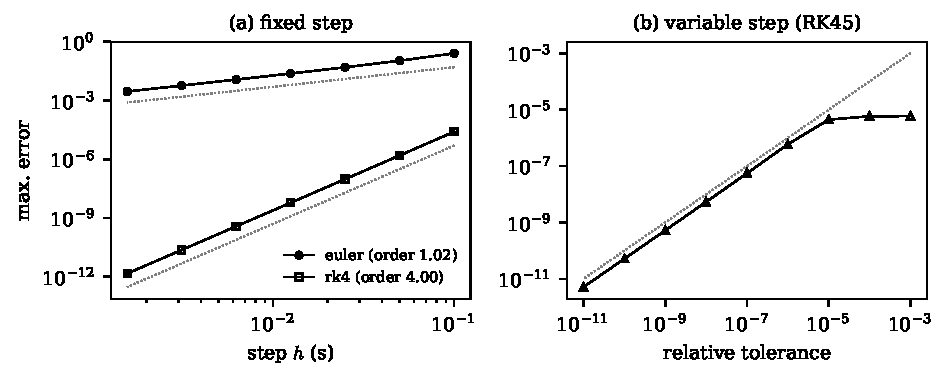
\includegraphics[width=\textwidth]{figures/convergence.pdf}}
  \caption{Convergence on the step response of the second-order system. (\textit{a}) Fixed-step solvers: largest
  error against the step $h$; dotted lines of slope 1 and 4. (\textit{b}) The default variable-step solver: largest
  error against the relative tolerance (absolute tolerance $10^{-2}$ times smaller); dotted line of slope 1. At
  tolerances looser than $10^{-5}$ the error is bounded by the default maximum step, a fiftieth of the run, rather
  than by the tolerance; the slope quoted in the text is fitted for tolerances of $10^{-6}$ and below.}
  \label{fig:convergence}
\end{figure}

\subsection{Solvers}

The step responses of a first- and a second-order linear system agree with their closed forms
to within the solver tolerance. Halving the step of the fixed-step solvers (figure~\ref{fig:convergence}\textit{a})
gives observed orders of \EulerOrder{} for explicit Euler and \RKOrder{} for classical Runge--Kutta, the
theoretical 1 and 4. The error of the variable-step solver falls with its tolerance with a log--log slope of
\RKFFSlope{} (figure~\ref{fig:convergence}\textit{b}).

\subsection{Events}

A body thrown upwards stops on the lower limit of its position integrator; the solver lands on
the exact impact time. For the integral of a sine clipped by a Saturation block, locating the clipping instants as
zero crossings gives an error of \SatErrOn{}; with zero-crossing detection switched off, the solver steps across
the kinks and the error is \SatErrOff{} at the same tolerance.

\subsection{Discrete and multirate}

The discrete PI loop of one of the Nervus tutorial models (a continuous motor,
a sampler and a discrete controller) has an exact sampled response: the motor discretized under a zero-order hold,
and the controller's own difference equations. The simulation reproduces it to round-off at 10~ms and 25~ms. The
loop becomes unstable when a closed-loop pole leaves the unit circle at $z=-1$, at $T = \StabExact$~ms; locating
the same limit from simulations alone, by the growth of the error from sample to sample, gives
$T = \StabSim$~ms.

\subsection{Physical networks}

Electrical (RC and series RLC), thermal, rotational and hydraulic networks, which
Nervus assembles from components connected by physical links rather than signals, reproduce their transients to
within the solver tolerance. The hydraulic case is a closed volume pressurized through a turbulent orifice with a
laminar core, $q = q_1\,\Delta p/\sqrt{|\Delta p| + p_{lam}}$, the pressure analogue of the draining tank of
\S\,\ref{sec:tank}; its separable equation has an implicit closed form, inverted by root-finding (half the supply
pressure is reached after \HydTHalf~s).

\subsection{Fluid analytics}

The two closed forms underlying the experimental cases are Torricelli draining of a
constant-area tank, $h(t)$ in \S\,\ref{sec:tank}, and the fall from rest of a sphere with a constant drag
coefficient and added mass, $v = v_t\tanh(t/T)$ and $z = v_t T\ln\cosh(t/T)$ with $v_t = (m_{app}g/k)^{1/2}$,
$T = m_{\mathrm{eff}}/(m_{app}g\,k)^{1/2}$ and $k = \frac12\rho C_D \upi d^2/4$, simulated with the same block
diagram as in \S\,\ref{sec:drops}.

\subsection{Linear analysis and code generation}

The Bode diagram of a first-order lag and the gain and phase
margins of three loops, two of them with poles at the origin, agree with their analytical values. Code generated
from a discrete controller (a PID with output limits and anti-windup, a discrete filter and a lookup table) and
compiled gives the same outputs as the simulation over \SilSteps{} random inputs to within \SilDiff{}, and a
fixed-point conversion to 16 bits with 8 fraction bits stays within \FixLSB{} of the least significant bit, the
half-LSB bound of rounding to nearest, both in simulation and in C.

%%%%%%%%%%%%%%%%%%%%%%%%%%%%%%%%%%%%%%%%%%%%%%%%%%%%%%%%%%%%%%%%%%%%%%%%%%%%%%%%%%%%%%%%%%%%%%%%%%%%%%%%%%%%%%%%%%
\section{Case 1: gravity draining of a tank through a side orifice}\label{sec:tank}

\subsection{Experiment}

\citet{Fabusola2025} drained water from an open plastic tank through a small circular hole drilled in its side and
recorded the water level with a resistive level strip read by a microcontroller every $0.16$~s. The tank is an
inverted, truncated cone with a rounded-rectangle cross-section; its inside height, measured along the wall, is
$h_{max} = 28.6$~cm. The
orifice has a radius $r_o = \Ro$~cm (a $5/64$~inch drill bit) and its centre is $h_o = 0.9$~cm above the base.
The length, width and perimeter of the top and bottom sections give the corner radii \RTop~cm and \RBottom~cm and
the areas \AreaTop~cm$^2$ and \AreaBottom~cm$^2$. We use the two experiments without an object in the tank: the
calibration run (\TrainN{} samples after the start of draining) and the replicate run (\TestN{} samples), both
from the authors' data repository \citep{FabusolaData}. Sensor counts are converted to levels with the authors'
calibration curve, a quadratic smoothing spline through 28 calibration points.

\subsection{Model}

Mass conservation, with Torricelli's law for the jet speed and a discharge coefficient $C_d$ for the contraction
and losses, gives the model used by \citet{Fabusola2025}:
\begin{equation}
  a(h)\,\frac{\mathrm{d}h}{\mathrm{d}t} = -C_d\,\upi r_o^2 \sqrt{2g\,(h-h_o)}, \qquad h(0) = h_0,
  \label{eq:tank}
\end{equation}
where $a(h) = lw + 2r(l+w) + \upi r^2$ is the area of a rounded rectangle whose length $l$, width $w$ and corner
radius $r$ vary linearly between their values at the bottom and at the top of the tank. In Nervus,
(\ref{eq:tank}) is a loop of eight blocks: an integrator for $h$; a sum for the head $h-h_o$; a saturation that
keeps it non-negative; a gain $2g$ and a square root for the jet speed; a gain $C_d\upi r_o^2$ for the flow
rate; a Python Function block for $a(h)$; and a product that divides the flow rate by the area. The
discharge coefficient is a workspace variable, so that the fit below changes it per run without rebuilding the
model.

\subsection{Data processing}

We follow the authors' processing \citep{FabusolaData}. Time zero is the instant of the highest sensor reading;
readings below 508 counts, \HCountsMin~cm, are discarded because the jet has then stopped and water runs down the
wall. The authors subsample each run to 20 points and omit the last three of the calibration run, because surface
tension stopped the outflow before the level reached the orifice. We use every sample, but end the calibration
window at the time of the authors' last retained point: $t = \TrainTcut$~s in the calibration run (level
\TrainHcut~cm) and, by the same rule, $t = \TestTcut$~s in the replicate run (\TestHcut~cm). The initial level
$h_0$ of each simulation is the first level of its own run: \TrainHzero~cm and \TestHzero~cm.

\subsection{Verification}

To separate numerical from modelling error, we first replace $a(h)$ by a constant $A = 120$~cm$^2$, for which
(\ref{eq:tank}) has the solution
\begin{equation}
  h(t) = h_o + \left( \sqrt{h_0-h_o} - \frac{C_d \upi r_o^2 \sqrt{2g}}{2A}\,t \right)^2 ,
\end{equation}
which reaches $h_o$ at $t = \VerTempty$~s for $h_0 = 25$~cm and $C_d = \Cfit$. Over 98\% of that time the largest
difference between the Nervus solution and the closed form is \VerAuto~cm with the default variable-step solver
and \VerRKfour~cm with fixed-step fourth-order Runge--Kutta and a 0.5~s step. For the real, variable-area tank,
the Nervus solution differs from an independent SciPy Radau solution at tolerance $10^{-11}$ by at most \VerScipy~cm.
Numerical error is therefore negligible against the centimetre-scale differences discussed below.

\subsection{Calibration and prediction}

Minimizing the sum of squared differences between the simulated and measured levels over the calibration window
(\TrainNfit{} samples) gives $C_d = \Cfit$. The fit depends little on where the window ends: ending it at 90\% and
75\% of $t = \TrainTcut$~s gives \CfitNinety{} and \CfitSeventyFive. The value lies within the broad prior
$0.65 \pm 0.25$ that \citet{Fabusola2025} took from \citet{Hicks2014}.

\begin{figure}
  \centerline{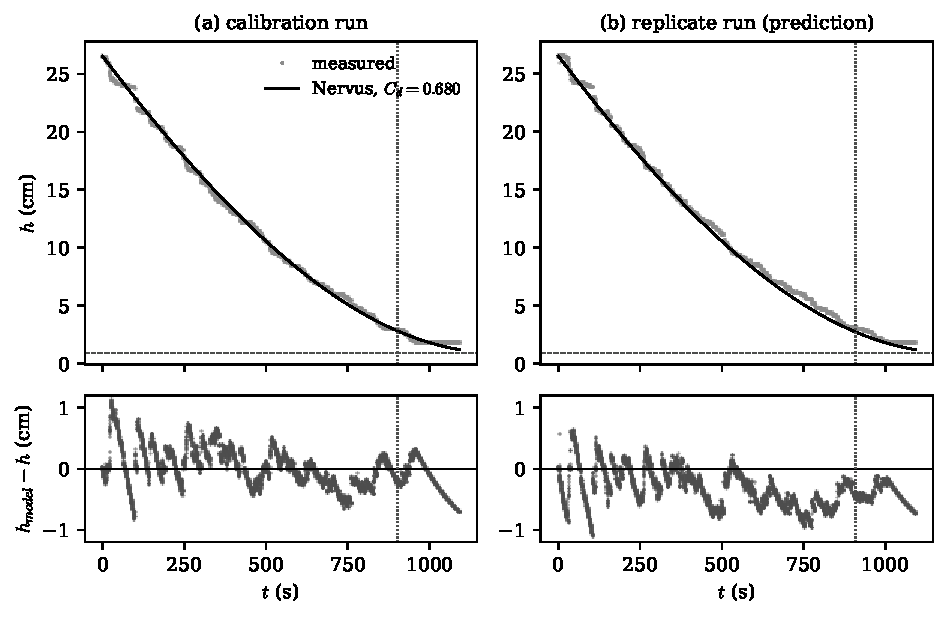
\includegraphics[width=\textwidth]{figures/tank.pdf}}
  \caption{Water level in the draining tank: measurements of \citet{Fabusola2025} (grey) and the Nervus model
  with $C_d$ fitted to the calibration run (black). (\textit{a}) Calibration run; (\textit{b}) replicate run,
  predicted with nothing refitted. The lower panels show the difference between model and measurement. The dotted
  line marks the end of the comparison window; the dashed line, the orifice height.}
  \label{fig:tank}
\end{figure}

\begin{table}
  \begin{center}
  \def~{\hphantom{0}}
  \begin{tabular}{lccccc}
    \toprule
    & samples & RMSE (cm) & MAE (cm) & max.\ $|e|$ (cm) & bias (cm) \\[3pt]
    \midrule
    calibration run, window & \TrainNfit & \TrainRMSE & \TrainMAE & \TrainMax & -- \\
    replicate run, window (prediction) & \TestNwin & \TestRMSE & \TestMAE & \TestMax & \TestBias \\
    replicate run, all samples & \TestN & \TestAllRMSE & \TestAllMAE & \TestAllMax & -- \\
    \bottomrule
  \end{tabular}
  \caption{Differences $e = h_{model} - h$ between the simulated and the measured level. Root-mean-square
  (RMSE), mean absolute (MAE) and largest absolute error; the bias is the mean of $e$.}
  \label{tab:tank}
  \end{center}
\end{table}

Figure~\ref{fig:tank} and table~\ref{tab:tank} show the result. The prediction of the replicate run has a
root-mean-square error of \TestRMSE~cm within the window and \TestAllRMSE~cm over all samples, which include the
final phase where surface tension holds the level above the orifice and the model, which has no surface tension,
keeps draining. On the authors' 20-point subsampling the mean absolute error is \TrainDSMAE~cm for the
calibration run (17 points) and \TestDSMAE~cm for the replicate run. \citet{Fabusola2025} report mean absolute
residuals of 0.26~cm and 0.29~cm for their Bayesian calibration, in which the tank dimensions, orifice size and
height and the initial level were also uncertain; with a single fitted parameter, the agreement here is of the
same order. The model reaches a level of 3~cm at \TrainTthreeModel~s and \TestTthreeModel~s, against
\TrainTthreeData~s and \TestTthreeData~s in the two runs.

\subsection{Structure of the residuals}

The residuals in figure~\ref{fig:tank} are not random: they form a saw-tooth that looks alike in both runs. Their
mean in 0.5~cm bins of level (figure~\ref{fig:resid}) has a correlation coefficient of \ResidCorr{} between the
two runs over \ResidBins{} bins. A model error that depended on time or on the flow history would not repeat at
the same levels in two experiments; an error in the level measurement would. The calibration points themselves
are uneven: the sensor reading rises by a median of \CalibStepMedian{} counts per centimetre of level, but by up to
\CalibStepMax{} counts between neighbouring points, and the smoothing spline through them misses the calibration
points by up to \CalibSplineMax~mm (root mean square \CalibSplineRMS~mm). We therefore attribute most of the
residual to the sensor calibration, and note that a fitted $C_d$ absorbs any systematic slope error of the
calibration curve.

\begin{figure}
  \centerline{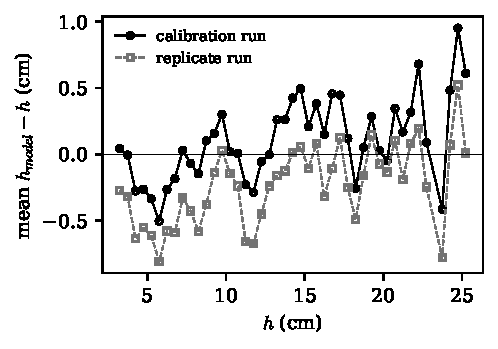
\includegraphics[width=0.55\textwidth]{figures/residual_h.pdf}}
  \caption{Mean difference between model and measurement in 0.5~cm bins of level, for the calibration and the
  replicate run, within the comparison window.}
  \label{fig:resid}
\end{figure}

\subsection{Caveats}

Only the product $C_d r_o^2$ is identified by the data. The measurement notes in the authors' repository
\citep{FabusolaData} give a hole diameter of $1/8$~inch and a hole height of 2.5~cm, whereas the paper and its
analysis code use $5/64$~inch and 0.9~cm; we follow the paper. With a $1/8$~inch hole the same data would give
$C_d = \CdEighth$, far below the value 0.65 for a round orifice \citep{Hicks2014} that \citet{Fabusola2025} used
as the centre of their prior, which supports the paper's dimensions. The level strip is mounted on the slanted wall, so it measures distance along the wall; from
the tape measurements of the top and bottom, the slant makes the vertical height shorter by a factor
\SlantFactor, a negligible correction. Water temperature was not
reported.

%%%%%%%%%%%%%%%%%%%%%%%%%%%%%%%%%%%%%%%%%%%%%%%%%%%%%%%%%%%%%%%%%%%%%%%%%%%%%%%%%%%%%%%%%%%%%%%%%%%%%%%%%%%%%%%%%%
\section{Case 2: Newton's falling spheres}\label{sec:drops}

\subsection{Experiments}

In the Scholium to Proposition~XL of Book~II of the \emph{Principia}, Newton tabulates two series of drops through
still air \citep{Newton1726}; we use the English translation of the 1846 edition \citep{Newton1846}. In June 1710
(Experiment~13; an account of drops from the same building is given by \citealt{Hauksbee1710}), pairs of glass
globes, one filled with mercury and one with air, were released together from a hinged table 220 English feet
(67.06~m) above the floor, and the fall was timed with a seconds pendulum. Newton subtracts about 0.3~s from the
times of the air-filled globes for the slow opening of the table; we compare with these corrected times. In July
1719 (Experiment~14), Desaguliers dropped hogs' bladders, blown up into spheres of about 5 inches, from 272 feet
(82.91~m) and timed them with half- and quarter-second pendulums. Newton notes that the bladders fluttered,
lengthening their falls by between half a second and a second, and that the fifth was wrinkled. A separate account
of Desaguliers's earlier drops of the same year is given by \citet{Desaguliers1719}. The tabulated weights were
taken in air, and times are given to a quarter or half second; for the mercury globes, only ``4'', ``4$^-$'' and
``4$^+$'' seconds.

\subsection{Model}

A sphere of diameter $d$ and volume $V = \upi d^3/6$, released from rest, obeys
\begin{equation}
  \left(m + \rho V + C_a \rho V\right) \frac{\mathrm{d}v}{\mathrm{d}t} = m_{app}\, g
  - \tfrac{1}{2}\rho\, C_D(Re)\, \frac{\upi d^2}{4}\, v|v|, \qquad
  \frac{\mathrm{d}z}{\mathrm{d}t} = v, \qquad Re = \frac{\rho v d}{\mu},
  \label{eq:drop}
\end{equation}
where $m_{app}$ is the tabulated weight in air, so that $m_{app}\,g$ is the weight less the buoyancy and
$m_{app} + \rho V$ is the mass, as Newton himself computed it; $C_a = 1/2$ is the added-mass coefficient of a
sphere in potential flow \citep{Batchelor1967}. For the drag coefficient we use the correlation of
\citet{Morrison2013}, intended for all Reynolds numbers up to $10^6$, in the form of \citet{Morrison2013handout}:
\begin{equation}
  C_D = \frac{24}{Re} + \frac{2.6\,(Re/5)}{1 + (Re/5)^{1.52}}
  + \frac{0.411\,(Re/263\,000)^{-7.94}}{1 + (Re/263\,000)^{-8.00}}
  + \frac{Re^{0.80}}{461\,000} .
  \label{eq:cd}
\end{equation}
A course sheet by the same author \citep{Morrison2013sheet} gives the fourth term as $0.25\,(Re/10^6)/(1+Re/10^6)$
and prints 236\,000 in place of the second 263\,000. The latter would give $C_D = \CdMisprintFiftyK$ at
$Re = 5\times10^4$, instead of \CdHandoutFiftyK, and contradicts the value 0.445 that the same sheet gives for
$10^3 \le Re \le 2.6\times10^5$; we take it to be a misprint.
The air density is Newton's own assumption, 1/860 of the density of rain water, $\rho = \RhoAir$~kg\,m$^{-3}$; the
viscosity is $\mu = 1.81\times10^{-5}$~Pa\,s. Nothing is fitted. In Nervus, (\ref{eq:drop}) is two integrators,
a constant for the net weight, a Python Function block for the drag and a gain for the inverse of the inertia;
the fall time is the time at which $z$ reaches the drop height, interpolated from the solution with a step of at
most 0.01~s.

To show how much the result depends on these choices, each drop is also simulated without added mass, with the
fourth term of \citet{Morrison2013sheet}, with the constant $C_D = 0.445$, and with air densities of 1.15 and
1.23~kg\,m$^{-3}$, those of dry air at 101.3~kPa and about \RhoTempHigh{} and \RhoTempLow~$^\circ$C; the air
temperature and pressure on the days of the experiments were not recorded.

\subsection{Results}

\begin{table}
  \begin{center}
  \def~{\hphantom{0}}
  \footnotesize
  \setlength{\tabcolsep}{2.5pt}
  \begin{tabular}{llrrccrrc}
    \toprule
    Exp. & object & $m_{app}$ (g) & $d$ (mm) & measured (s) & Nervus (s) & error (s) & $Re/10^4$ &
    $C_{D,\mathrm{eff}}$ \\[3pt]
    \midrule
    \StPaulsRows
    \bottomrule
  \end{tabular}
  \caption{Fall times from St~Paul's Cathedral. Measured: Newton's table; for the 1710 glass globes, the observed
  time with Newton's corrected time in brackets. Nervus: (\ref{eq:drop}) with (\ref{eq:cd}); figure~\ref{fig:drops}(\textit{a}) shows
  the spread over the sensitivity runs described in the text. Error: Nervus minus the (corrected) measured time. $Re$: at
  impact. $C_{D,\mathrm{eff}}$: the constant drag coefficient with which the simulated fall takes the measured
  time.}
  \label{tab:drops}
  \end{center}
\end{table}

\begin{figure}
  \centerline{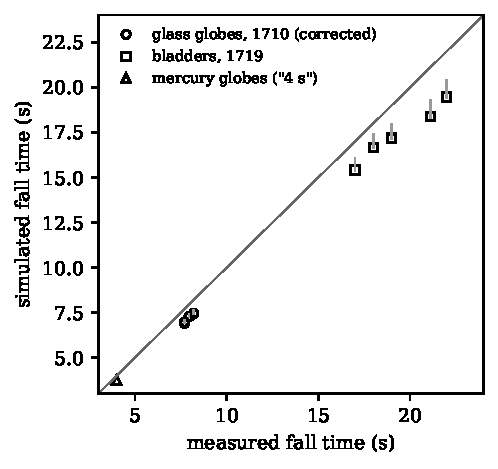
\includegraphics[width=0.5\textwidth]{figures/stpauls.pdf}
              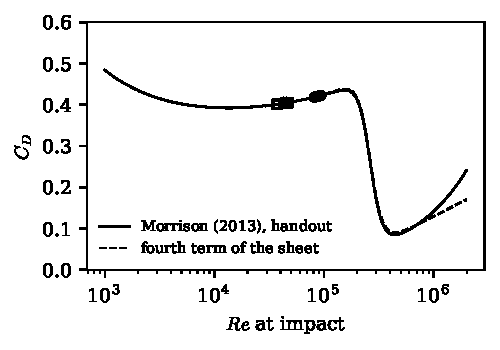
\includegraphics[width=0.5\textwidth]{figures/cd.pdf}}
  \caption{(\textit{a}) Simulated against measured fall times; the vertical bars span the sensitivity runs.
  (\textit{b}) The drag correlation (\ref{eq:cd}) (solid) and the same with the fourth term of
  \citet{Morrison2013sheet} (dashed), with the drag coefficient of each object at impact.}
  \label{fig:drops}
\end{figure}

Table~\ref{tab:drops} and figure~\ref{fig:drops} compare the simulated and measured times. The model is
systematically fast. For the six air-filled globes the mean error is \GlobeMeanErr~s (\GlobeRel\%) and the
largest \GlobeMax~s; for the five bladders the mean error is \BladderMeanErr~s (\BladderRel\%) and the largest
\BladderMax~s. Every light object is predicted to land early, by more than the quarter- to half-second resolution
of the timing. The mercury globes, which fall almost as in vacuum (\TvacThirteen~s without air), are predicted to
take \MercT~s, against Newton's ``4'', ``4$^-$'' and ``4$^+$'' seconds; their times were not corrected for
the release of the table, which Newton estimated at about 0.3~s for the air-filled globes.

The discrepancy is not an artefact of the modelling choices: the sensitivity runs (no added mass, the other form
of the correlation, a constant $C_D = 0.445$, air densities from 1.15 to 1.23~kg\,m$^{-3}$) lengthen the
globes' falls by at most \GlobeSensUp~s, against a shortfall of at least \GlobeMinDeficit~s, and the bladders'
by at most \BladderSensUp~s, against at least \BladderMinDeficit~s; \SensReachedText. Nor is the discrepancy
numerical. Expressed as drag, it is the difference between
the correlation's $C_D \approx \GlobeCdModel$ at impact and an effective constant coefficient of \GlobeCdEff{}
(\GlobeCdEffMin--\GlobeCdEffMax) for the globes, \GlobeCdRatio\% higher; for the bladders, between
\BladderCdModel{} and \BladderCdEff{} (\BladderCdEffMin--\BladderCdEffMax), \BladderCdRatio\% higher.
Because the light objects reach 95\% of their terminal speed within the first \GlobeTninetyFive\% (globes) and
\BladderTninetyFive\% (bladders) of the fall, these effective coefficients are close to the terminal-speed drag
and depend little on the initial acceleration, added mass or history forces.

The Reynolds numbers at impact are $(\GlobeReMin\text{--}\GlobeReMax)\times10^4$ for the glass globes and
$(\BladderReMin\text{--}\BladderReMax)\times10^4$ for the bladders, in the subcritical range where the drag
coefficient of a smooth sphere is nearly constant; the drag crisis occurs at Reynolds numbers of a few times
$10^5$ \citep{Achenbach1972}. The results therefore do not depend on the details of the correlation near the
crisis, as the sensitivity runs confirm. For the bladders, the flutter that Newton describes adds drag and
lateral motion that (\ref{eq:drop}) leaves out, and Newton's own estimate of its effect, half a second to a
second, accounts for part of their \BladderMeanErr~s. For the rigid glass globes no such explanation is offered by
the sources. Total fall times alone cannot separate the remaining candidates: a systematic error in the timing or
the release, air movement in the dome, the globes' surface and shape, or drag on a freely falling sphere that is
higher than on a fixed sphere in a steady stream.

%%%%%%%%%%%%%%%%%%%%%%%%%%%%%%%%%%%%%%%%%%%%%%%%%%%%%%%%%%%%%%%%%%%%%%%%%%%%%%%%%%%%%%%%%%%%%%%%%%%%%%%%%%%%%%%%%%
\section{Discussion}\label{sec:discussion}

In both cases the numerical error of the simulator is orders of magnitude smaller than the differences between
model and measurement, so the comparison tests the lumped models and the data rather than the integration. The
differences have identifiable sources. In the tank, the residuals are dominated by the level-sensor calibration,
as their repetition at the same levels in two runs shows; the remaining model error comes from treating $C_d$ as
constant, although it can depend on the Reynolds number of the jet, which falls with the head (see the discussion
and references in \citealt{Fabusola2025}), and from neglecting surface tension, which ends the outflow before the level reaches the orifice. In the drops, the
measurements are coarse (a quarter to half a second), the air density was not recorded, the release of the 1710
globes needed a correction, and the bladders were neither rigid nor spherical. Here the comparison does find a
discrepancy: a steady-sphere correlation without fitted parameters predicts fall times about 10\% short, a
difference that the uncertainties in the model's inputs cannot explain. For a simulator, this is the useful
outcome of a validation: the numerics are exact to the precision that matters, and the remaining difference
points at the physics put into the model.

Zero-dimensional models leave out what this comparison cannot see: the velocity field inside the tank, the vena
contracta and its dependence on the orifice edge, unsteady wake forces on an accelerating sphere beyond the
added mass, and lateral motion. A natural next step for the tank case would be a model of the sensor itself,
calibrated on the static calibration points, and for the methodology a benchmark in which the physical parameters
are unknown and must be identified, such as the cascaded-tanks data of \citet{Schoukens2017}.

%%%%%%%%%%%%%%%%%%%%%%%%%%%%%%%%%%%%%%%%%%%%%%%%%%%%%%%%%%%%%%%%%%%%%%%%%%%%%%%%%%%%%%%%%%%%%%%%%%%%%%%%%%%%%%%%%%
\section{Conclusions}\label{sec:conclusions}

We have verified the block-diagram simulator Nervus against exact solutions, module by module, and compared
lumped fluid models built with it with two published data sets.
For the draining tank, one discharge coefficient fitted to one run predicts a replicate run to within
\TestRMSE~cm root-mean-square over a \LevelDrop~cm drop in level, with residuals that are traceable to the level sensor.
For Newton's falling spheres, a published steady-sphere drag correlation without any fitted parameter predicts
falls that are too short, by \GlobeRel\% for the glass globes and \BladderRel\% for the bladders on average,
which corresponds to effective drag coefficients about \GlobeCdRatio\% and \BladderCdRatio\% above the
correlation; the
bladders' flutter explains part of their difference, the globes' remains open. The scripts, models and processed results are
available so that the comparison can be repeated with later versions of the simulator.

%%%%%%%%%%%%%%%%%%%%%%%%%%%%%%%%%%%%%%%%%%%%%%%%%%%%%%%%%%%%%%%%%%%%%%%%%%%%%%%%%%%%%%%%%%%%%%%%%%%%%%%%%%%%%%%%%%
\backsection[Data and code availability]{The tank data are those of \citet{Fabusola2025}, available from
\url{https://github.com/SimonEnsemble/tank_inverse_problem}; they are not redistributed here. Newton's table is
public domain and is included as \texttt{newton1726\_st\_pauls.csv}. The analysis script \texttt{analysis.py},
which builds every Nervus model and produces every figure and number in this paper (\texttt{results.json}),
accompanies this manuscript and is to be deposited with the Nervus source code \citep{Nervus}.}

\backsection[Acknowledgements]{We thank G. Fabusola and C. M. Simon for publishing their measurements and
analysis code, and the volunteers of Wikisource for the transcription of the 1846 edition of the
\emph{Principia}.}

\backsection[Funding]{[To be completed by the authors.]}

% JFM requires a declaration of interests. Placeholder, to be confirmed by both authors:
% \backsection[Declaration of interests]{The authors report no conflict of interest.}

\backsection[Author contributions]{[To be completed by the authors.]}

\bibliographystyle{jfm}
\bibliography{references}

\end{document}
